\let\negmedspace\undefined
\let\negthickspace\undefined
\documentclass[journal]{IEEEtran}
\usepackage[a5paper, margin=10mm, onecolumn]{geometry}
\usepackage{tfrupee}

\setlength{\headheight}{1cm}
\setlength{\headsep}{0mm}

\usepackage{gvv-book}
\usepackage{gvv}
\usepackage{cite}
\usepackage{amsmath,amssymb,amsfonts,amsthm}
\usepackage{algorithmic}
\usepackage{graphicx}
\usepackage{textcomp}
\usepackage{xcolor}
\usepackage{txfonts}
\usepackage{listings}
\usepackage{enumitem}
\usepackage{mathtools}
\usepackage{gensymb}
\usepackage{comment}
\usepackage[breaklinks=true]{hyperref}
\usepackage{tkz-euclide} 
\usepackage{listings}

\graphicspath{{./figs/}}

\begin{document}
\title{4.4.6}
\author{AI25BTECH11010 - Dhanush Kumar}
\maketitle
\renewcommand{\thefigure}{\theenumi}
\renewcommand{\thetable}{\theenumi}

\noindent
\textbf{Question:}\\
Find the equation of the plane passing through the points 
$A(2, 5, -3), B(-2, -3, 5)$ and $C(5, 3, -3)$.
\bigskip

\noindent
\textbf{Solution:}\\

\begin{align}
\vec{A} &= \myvec{2 \\ 5 \\ -3}, & 
\vec{B} &= \myvec{-2 \\ -3 \\ 5}, & 
\vec{C} &= \myvec{5 \\ 3 \\ -3}.
\end{align}

Let the equation of the plane be
\begin{align}
\vec{n}^T \vec{x} &= 1.
\end{align}

Since $\vec{A}, \vec{B}, \vec{C}$ lie in the plane:
\begin{align}
\vec{n}^T \vec{A} &= 1, & 
\vec{n}^T \vec{B} &= 1, & 
\vec{n}^T \vec{C} &= 1,
\end{align}
or equivalently
\begin{align}
\vec{A}^T \vec{n} &= 1, & 
\vec{B}^T \vec{n} &= 1, & 
\vec{C}^T \vec{n} &= 1.
\end{align}

Hence,


\begin{align}
\myvec{\vec{A} & \vec{B} & \vec{C}}^{T} \vec{n} 
&= 1.
\end{align}
\begin{align}
\myvec{ 2 & 5 & -3 \\ -2 & -3 & 5 \\ 5 & 3 & -3}\vec{n}
&= \myvec{1 \\ 1 \\ 1}.
\end{align}

Performing row operations:
\begin{align}
R_2 &\leftarrow R_2 + R_1, \\
\myvec{2 & 5 & -3 \\ 0 & 2 & 2 \\ 5 & 3 & -3}\vec{n}
&= \myvec{1 \\ 2 \\ 1},\\
R_3 &\leftarrow 2R_3 - 5R_1, \\
\myvec{2 & 5 & -3 \\ 0 & 2 & 2 \\ 0 & -19 & 9}\vec{n}
&= \myvec{1 \\ 2 \\ -3},\\ 
R_3 &\leftarrow 19R_2 + 2R_3, \\
\myvec{2 & 5 & -3 \\ 0 & 2 & 2 \\ 0 & 0 & 56}\vec{n}
&= \myvec{1 \\ 2 \\ 32}.
\end{align}

Thus, solving we get
\begin{align}
\vec{n} = \myvec{\tfrac{2}{7} \\ \tfrac{3}{7} \\ \tfrac{4}{7}}.
\end{align}
Therfore,
The equation of plane is
\begin{align}
	\myvec{\tfrac{2}{7} \\ \tfrac{3}{7} \\ \tfrac{4}{7}}^T\vec{x} &= 1.
\end{align}
\begin{figure}[h!]
  \centering
   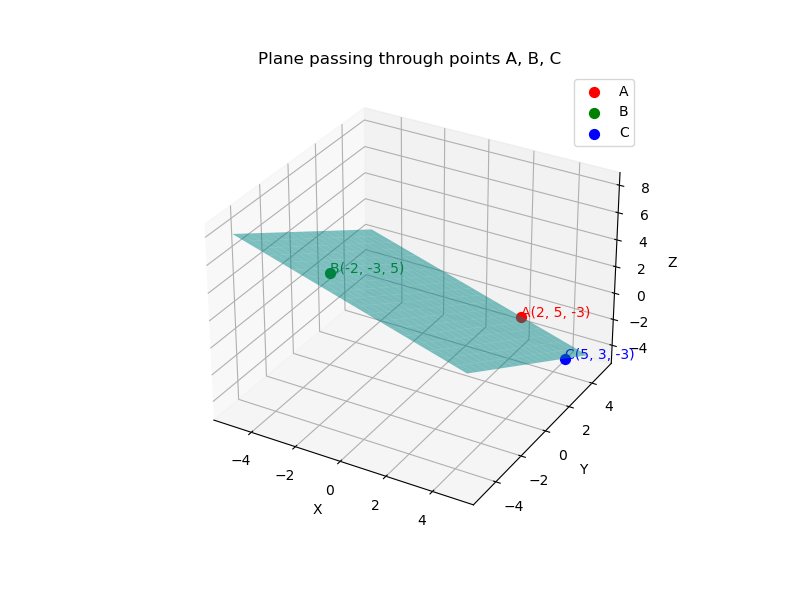
\includegraphics[width=0.7\linewidth]{../figs/plane_plot.png}
   \caption{}
  \label{stemplot}
\end{figure}

\end{document}
